\chapter{Tema 7: Predicción estructurada. Modelos ocultos de Markov}

\section{Introducción}

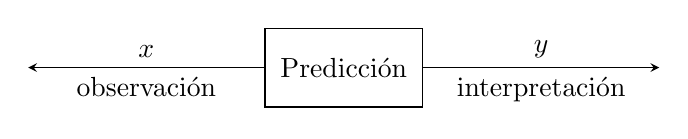
\begin{tikzpicture}[>=stealth]
    % Draw the rectangular box
    \node[draw, minimum width=2cm, minimum height=1cm, align=center] (box) {Predicción};
    
    % Draw the left arrow and label
    \draw[->] (box.west) -- ++(-3,0) node[midway, above] {$x$} node[midway, below] {observación};
    
    % Draw the right arrow and label
    \draw[->] (box.east) -- ++(3,0) node[midway, above] {$y$} node[midway, below] {interpretación};
\end{tikzpicture}

\section{Aplicaciones}

\begin{itemize}
    \item Natural Language Processing (NLP)
    \begin{itemize}
        \item Part-of-speech tagging
        \item Parsing
        \item Machine translation
        \item Information extraction
    \end{itemize}
    \item Procesamiento de imágenes
    \begin{itemize}
        \item Reconocimiento de caracteres
        \item Análisis visual de escenas
    \end{itemize}
    \item Procesamiento de voz
    \begin{itemize}
        \item Transcripción automática
        \item Texto a voz
    \end{itemize}
    \item Bioinformática
    \begin{itemize}
        \item Predicción de la estructura de proteínas
    \end{itemize}
    \item Robótica
    \begin{itemize}
        \item Localización y mapeo simultáneos (SLAM)
        \item Planificación de trayectorias
    \end{itemize}
\end{itemize}

\section{Espacio de búsqueda}

$\mathcal{Y}$ es potencialmente infinito, por lo que $f(x) = y \in \mathcal{Y}$
será intratable.

\section{Lenguajes: Definiciones básicas}

\section{Modelos aceptores: Autómatas}

\subsection{Autómata finito determinista (DFA)}

Es una tupla $A = (\Sigma, Q, \delta, q_0, F)$ donde:

\begin{itemize}
    \item $\Sigma$ es el alfabeto de entrada
    \item $Q$ es el conjunto finito y no vacío de estados del autómata
    \item $\delta$ es la función de transición entre estados $Q \times \Sigma \to Q$
    \item $q_0 \in Q$ es el estado inicial
    \item $F \subseteq Q$ es el conjunto de estados finales
\end{itemize}

$\delta$ es una matriz de transición de tamaño $|Q| \times |\Sigma|$.
Cada fila de la matriz representa un estado y cada columna representa un símbolo
del alfabeto. Cada celda contiene el estado al que se transita desde el estado
correspondiente al número de fila al leer el símbolo correspondiente al número
de columna.

\begin{examplebox}{Ejemplo de autómata}
    \begin{equation*}
        A = (\Sigma = {a, b}, Q = {0, 1, 2}, \delta, q_0 = 0, F = {2})
    \end{equation*}
\end{examplebox}

Para el ejemplo anterior, la matriz de transición sería:

\begin{align*}
    \left[
    \begin{array}{cc}
        1 & 0 \\
        2 & 1 \\
        2 & 2
    \end{array}
    \right]
\end{align*}

\section{Equivalencia de modelos}

\begin{definitionbox}{Equivalencia de modelos}
    Dos modelos, $M_1$ y $M_2$, son equivalentes si definen
    (aceptan o generan) el mismo lenguaje.

    $$ M_1 \equiv M_2 \iff L(M_1) = L(M_2) $$
\end{definitionbox}

\textbf{Teorema.} Dada una gramática regular, $G$, se puede construir un autómata
finito determinista, $A$, tal que $L(G) = L(A)$.

\section{Incertidumbre}

\section{Lenguaje probabilístico}

\textbf{Lenguaje}    $L \subseteq \Sigma^*$, dado un alfabeto $\Sigma$.

\textbf{Lenguaje generado por una gramática}    $L \subseteq \Sigma^*$, dado un
alfabeto $\Sigma$ y una gramática $G = (N,\Sigma S, \mathcal{P})$.
$$ L(G) = \{ x | x \in \Sigma^* : S \Rightarrow^+ x \} $$

\section{Gramáticas Regulares Probabilísticas}

Se expresa como $G_\theta = (G, P)$, donde

\begin{itemize}
    \item $G = (N, \Sigma, S, \mathcal{P})$ es una gramática regular característica
    \item $P : \mathcal{P} \to [0, 1]$ es una función de probabilidad
\end{itemize}

\section{Ejercicios}

\subsection{Ejercicio 1}
\begin{exercisebox}{Ejercicio 1}

    \[
    G = (N = \{S, A, B\}, \, \Sigma = \{a, b\}, \, S, \, P)
    \]
    
    \[
    P = 
    \begin{cases}
    S \to aA \mid bB \mid b \\
    A \to aA \mid bB \mid b \\
    B \to bB \mid b
    \end{cases}
    \]

\end{exercisebox}

\subsubsection*{Apartado 1}

Sí que es una gramática regular, ya que todas las producciones son de la forma
$A \to aB$ o $A \to a$, donde $A$ y $B$ son no terminales y $a$ es un terminal.

\subsubsection*{Apartado 2}
Primero:
El primer símbolo de la secuencia es un no terminal B, por lo que no se puede
haber generado con esta gramática.

Segundo:
No se puede generar la secuencia $bA$ con esta gramática.

Tercero:
Se podría generar a través de la producción $S \to aA \quad A \to bB$.

Cuarto:
Se podría generar a través de la producción $S \to bB \quad B \to b$.

\subsubsection*{Apartado 3}

Primero:
Se genera a partir de la siguiente secuencia de producciones:
$$S \to aA \to aaA \to aaaA \to aaabB \to aaabb$$
Segundo:
No se podría generar, ya que no se puede generar una $b$ después de una $a$.

Tercero:
Se genera a partir de la siguiente secuencia de producciones:
$$ S \to aA \to ab $$

Cuarto:
No se puede generar por lo mismo que en el segundo apartado.

\subsection{Ejercicio 2}

\begin{exercisebox}{Ejercicio 2}


    \begin{enumerate}
        \item ¿Cuál es la longitud mínima de la cadena de símbolos que puede
        aceptar?
        \item ¿Cuáles serían las cadenas de mínima longitud que puede aceptar?
        \item ¿Dicho autómata aceptaría las cadenas del tipo $a^n b^m c^n$, con
        $n > 0$ y $m > 0$?
        \item ¿Cuál sería la gramática regular equivalente?
    \end{enumerate}
\end{exercisebox}

\subsubsection*{Apartado 1}

La longitud mínima es 1, ya que se puede llegar a un estado final (2 o 3)
desde el estado inicial.

\subsubsection*{Apartado 2}

Las cadenas de mínima longitud que puede aceptar son $b$ y $c$.

\subsubsection*{Apartado 3}

El autómata sí podría aceptar cadenas del tipo $a^n b^m c^n$, ya que se
puede repetir el símbolo $a$ y el símbolo $b$ y el símbolo $c$ tantas
veces como se quiera en la misma cadena.

\subsubsection*{Apartado 4}

La gramática regular equivalente sería:


\[
P = 
\begin{cases}
S \to aS \mid bA \mid b \mid cB \mid c \\
A \to bA \mid b \mid cB \mid c \\
B \to cB \mid c
\end{cases}
\]

Donde $S$ es el estado inicial (1), $A$ es el estado final 2 y $B$ es el
estado final 3.

\subsection{Ejercicio 3}

\begin{exercisebox}{Ejercicio 3}
    Dada la gramática regular probabilística, ¿cuál será la probabilidad de la
    interpretación más probable para la cadena de entrada $a \, b \, a \, b$?
    \[
    \begin{aligned}
    S &\rightarrow aS \quad 0.3 \quad &| \quad A &\rightarrow bA \quad 0.2 \\
    S &\rightarrow bS \quad 0.2 \quad &| \quad A &\rightarrow aA \quad 0.2 \\
    S &\rightarrow bA \quad 0.3 \quad &| \quad A &\rightarrow aS \quad 0.1 \\
    S &\rightarrow b \quad 0.2  \quad &| \quad A &\rightarrow b \quad 0.5
    \end{aligned}
    \]
\end{exercisebox}

Forma 1:

\[
S \overset{\textcolor{green}{0.3}}{\longrightarrow} aS 
\overset{\textcolor{green}{0.2}}{\longrightarrow} abS 
\overset{\textcolor{green}{0.3}}{\longrightarrow} abaS 
\overset{\textcolor{green}{0.2}}{\longrightarrow} abab
\]

Probabilidad: $0.3 \cdot 0.2 \cdot 0.3 \cdot 0.2 = 0.0036$

\textbf{Forma 2:}

\[
S \overset{\textcolor{green}{0.3}}{\longrightarrow} aS 
\overset{\textcolor{green}{0.3}}{\longrightarrow} abA 
\overset{\textcolor{green}{0.2}}{\longrightarrow} abaA 
\overset{\textcolor{green}{0.5}}{\longrightarrow} abab
\]

Probabilidad: $0.3 \cdot 0.3 \cdot 0.2 \cdot 0.5 = 0.009$

\textbf{Forma 3:}

\[
S \overset{\textcolor{green}{0.3}}{\longrightarrow} aS 
\overset{\textcolor{green}{0.3}}{\longrightarrow} abA 
\overset{\textcolor{green}{0.1}}{\longrightarrow} abaS 
\overset{\textcolor{green}{0.2}}{\longrightarrow} abab
\]

Probabilidad: $0.3 \cdot 0.3 \cdot 0.1 \cdot 0.2 = 0.0018$

\subsection{Ejercicio 4. Ejercicio de examen}

Probabilidad de transición:
\[
\begin{array}{|c|c|c|c|c|}
\hline
\textbf{Prob. Transición} & 1 & 2 & 3 & F \\ \hline
1 & 0.8 & 0.2 & 0.0 & 0.0 \\ \hline
2 & 0.0 & 0.6 & 0.3 & 0.1 \\ \hline
3 & 0.4 & 0.0 & 0.5 & 0.1 \\ \hline
\end{array}
\]

Probabilidad de emisión:
\[
\begin{array}{|c|c|c|}
\hline
\textbf{Prob. Emisión} & a & b \\ \hline
1 & 0.3 & 0.7 \\ \hline
2 & 0.0 & 1.0 \\ \hline
3 & 0.6 & 0.4 \\ \hline
\end{array}
\]

\begin{exercisebox}{Ejercicio examen}
    \begin{enumerate}[label=\alph*)]
        \item Representad gráficamente este modelo.
        
        \item Calculad la probabilidad de que el modelo genere la cadena \texttt{abbba} a través de la secuencia de estados $31223$.
        
        \item Completad la traza del algoritmo de Viterbi para obtener la secuencia de estados más probable con la que el modelo da cuenta de la cadena \texttt{abb}. Obtened además la probabilidad resultante (probabilidad de Viterbi).
        
        \item Estimad los parámetros de $M$ mediante una iteración de estimación por Viterbi, a partir de los siguientes pares (cadena, secuencia óptima de estados):
        \[
        \begin{array}{l}
        \text{cadenas} \quad \texttt{abbba} \quad \texttt{bbba} \quad \texttt{bba} \\
        \text{estados} \quad 31223 \quad 1223 \quad 333
        \end{array}
        \]
        
        Además, también se debe añadir la cadena \texttt{abb} y la secuencia óptima de estados obtenida en el apartado anterior (total 4 pares).
    \end{enumerate}
\end{exercisebox}

\subsubsection{Apartado a}

Está dibujado en el ipad.

\subsubsection{Apartado b}

Para obtener la cadena \texttt{abbba} usando viterbi a través de \texttt{31223},
se puede hacer de la siguiente forma:

\begin{enumerate}
    \item $I \to 3 \quad \text{Probabilidad(a)} = 0.2 \cdot 0.6 = 0.12$
    \item $3 \to 1 \quad \text{Probabilidad(b)} = 0.12 \cdot 0.4 \cdot 0.7 = 0.0336$
    \item $1 \to 2 \quad \text{Probabilidad(b)} = 0.0336 \cdot 0.2 \cdot 1 = 0.00672$
    \item $2 \to 2 \quad \text{Probabilidad(b)} = 0.00672 \cdot 0.6 \cdot 1 = 0.004032$
    \item $2 \to 3 \quad \text{Probabilidad(b)} = 0.004032 \cdot 0.3 \cdot 0.4 = 0.0012096$
    \item $3 \to F \quad \text{Probabilidad(b)} = 0.0012096 \cdot 0.1 = 0.00012096$
\end{enumerate}

Resultado = $0.000217728$

\subsubsection{Apartado c}

\[
\begin{array}{|c|c|c|c|c|}
\hline
& a & b & & \\ \hline
1 & 0.12 & 
\begin{array}{l}
1: 0.0672 \\
3: 0.1008
\end{array} & & \\ \hline
2 & \emptyset & 
\begin{array}{l}
1: 0.0240 \\
2: \emptyset
\end{array} & & \\ \hline
3 & 0.36 & 
\begin{array}{l}
2: \emptyset \\
3: 0.072
\end{array} & & \\ \hline
F & & & & \\ \hline
\end{array}
\]


\subsubsection{Apartado d}

\[
\begin{array}{l}
\text{cadenas} \quad \texttt{abbba} \quad \texttt{bbba} \quad \texttt{bba} \quad \texttt{abb} \\
\text{estados} \quad 31223F \quad 1223F \quad 333F \quad 321F
\end{array}
\]

\begin{itemize}
    \item Veces que se transita del estado 1 al estado 1: 0
    \item Veces que se transita del estado 1 al estado 2: 1
    \item Veces que se transita del estado 1 al estado 3: 0
    \item Veces que se transita del estado 1 al estado F: 1
    \item Veces que se transita del estado 2 al estado 1: 0
    \item Veces que se transita del estado 2 al estado 2: 2
    \item Veces que se transita del estado 2 al estado 3: 1
\end{itemize}